%
% $RCSfile: singleton.tex,v $
%
% Copyright (C) 2002-2008. Christian Heller.
%
% Permission is granted to copy, distribute and/or modify this document
% under the terms of the GNU Free Documentation License, Version 1.1 or
% any later version published by the Free Software Foundation; with no
% Invariant Sections, with no Front-Cover Texts and with no Back-Cover
% Texts. A copy of the license is included in the section entitled
% "GNU Free Documentation License".
%
% http://www.cybop.net
% - Cybernetics Oriented Programming -
%
% http://www.resmedicinae.org
% - Information in Medicine -
%
% Version: $Revision: 1.1 $ $Date: 2008-08-19 20:41:08 $ $Author: christian $
% Authors: Christian Heller <christian.heller@tuxtax.de>
%

\subsubsection{Singleton}
\label{singleton_heading}
\index{Singleton Pattern}
\index{Global Data Access}
\index{Class Method}
\index{Registry Object Pattern}
\index{Manager Object Pattern}
\index{Lifecycle Method}

Whenever an object-oriented system wants to ensure that only one instance of a
certain class exists, the \emph{Singleton} pattern \cite{gamma1995} can be
used. It essentially is a class which encapsulates its instance's data and
provides global access to them, via \emph{static}, sometimes called
\emph{class} methods (figure \ref{singleton_figure}).

\begin{figure}[ht]
    \begin{center}
        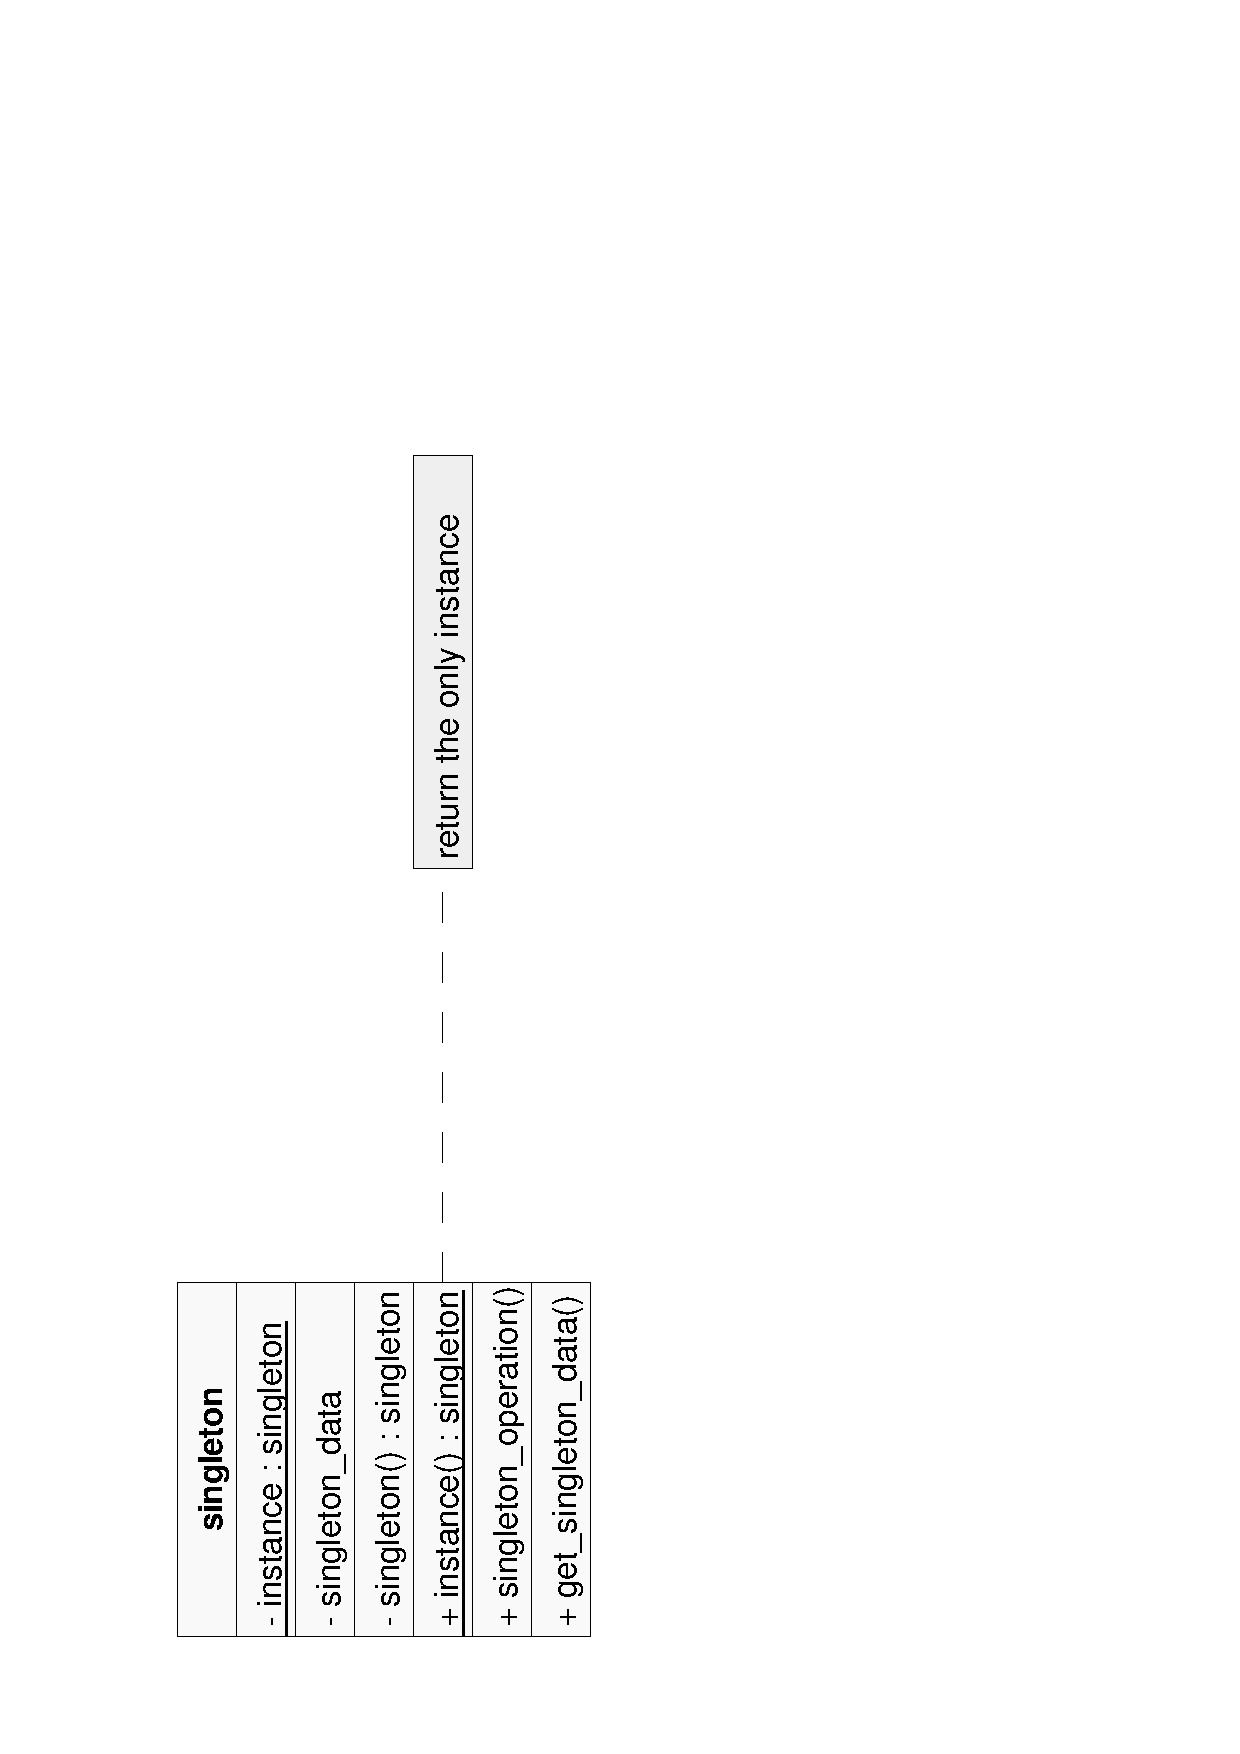
\includegraphics[scale=0.3,angle=-90]{graphic/singleton.pdf}
        \caption{Singleton Pattern}
        \label{singleton_figure}
    \end{center}
\end{figure}

A \emph{Registry} object as described by Fowler \cite{fowler2002} often uses
the \emph{Singleton} pattern, to be unique and to become globally accessible.
Similarly do many so-called \emph{Manager} objects, for example change managers
which are also responsible for the caching of objects.

Global, that is static access -- the main purpose of the \emph{Singleton}
pattern, is its main weakness, at the same time. One obvious solution to avoid
singleton objects could be to forward global information as instances from
component to component, possibly using an own \emph{Lifecycle Method} (section
\ref{component_lifecycle_heading}). This approach, however, might bring with a
rather large number of parameters to be handed over. It therefore seems easier
to use another alternative -- the central tree of knowledge instances, as done
in the interpreter of chapter \ref{cybernetics_oriented_interpreter_heading}.
